%!TEX root = main.tex
\chapter{Views}

% What is a view? Referere til kapittel 9

Different views support different goals and uses.
The views you should document depend on the uses you expect to make of the documentation.

% Relevant views

% Fremgangsmåte
% 1. Produce a candidate view list
% 2. Combine views
% 3. Prioritize

As described in chapter \ref{cha:architectural_viewpoint}, the views deemed the most useful for the development of LaHAW is the \emph{logic}, \emph{development} and \emph{process} views from the 4+1 view model.
In addition to these views there is the \emph{physical} and the \emph{scenario} view. We have decided to not detail these views.



\section{Logic view}

% 1. Primariy presentation
% 2. Element catalog
% 3. Context diagram
% 4. Variability
% 5. Architecture background
% 6. Glossary of terms
% 7. Other information

\begin{figure}[ht]
	\centering
    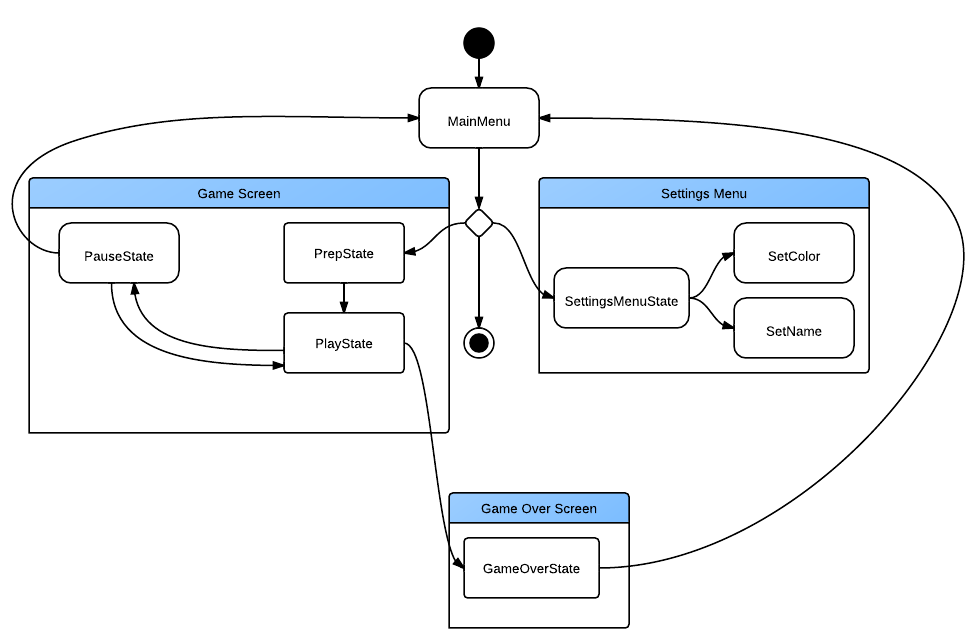
\includegraphics[width=\textwidth]{LogicView.png}
    \caption{UML Class diagram illustrating the Logical View}
    \label{fig:LogicalView}
\end{figure}

Figure \ref{fig:LogicalView} shows a simplified overview of the different classes and their uses. The notation is based on the Logical View notation by Kruchten\cite{kruchten}. This decomposition helps identify elements that are shared across the system.

\texttt{GameOverState}, \texttt{PrepState} and \texttt{PlayState} all extend a common \texttt{State} class (not shown here), and describes the different states the game can exist in at a given time.

% A state machine class (not shown here) functions as the game's main controller, and controls the state stack. The \texttt{Ship} object instantiates the different ship types with a given set of attributes, which in turn is controlled by the main \texttt{Game} class.

Other states and objects, such as warships and ocean space, are discussed earlier in this report, but are not represented in this diagram. The main reason for this decision is to keep the diagram simple and easy to read, and that the ignored features are either redundant or too specific.



\section{Development view}


\begin{figure}[ht]
	\centering
    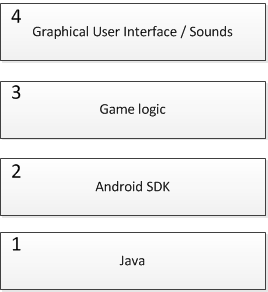
\includegraphics[scale=0.65]{DevelopmentView.png}
    \caption{Development View Architecture Layer Diagram}
    \label{fig:DevelopmentView}
\end{figure}

Figure \ref{fig:DevelopmentView} illustrates the different layers that the developers needs to take into account when developing the application. We used a three layered approach which separate the underlying operating system and COTS from our own logic layer and the assets used by our code. If implemented properly, this will make it possible to completely rework or replace one or more of the layers to port or maintain the code, without interfering with what is done in other layers.

This will aid the maintainability, as separating the different parts of the code base into layers will make it possible to change and maintain and not break code in different layers.

% Additionally, this will aid the portability of the game. If the game is to be ported to Apple iOS, we can replace the lowermost layers, keeping the uppermost GUI and sound layer, adapting the game logic code to use the new API.

This will help the application by making it possible for the developers to implement the different subsystems in tandem. This requires that each of the layers properly provides a well-defined interface to the layers above it. In this application, the code that directly interfaces with Android has to provide an API for the graphical layer above it, that it can use even though the internal algorithms behind the APIs are in flux.


\section{Process view}
% Non-functional requirements - performance, availability
    
\begin{figure}[ht]
    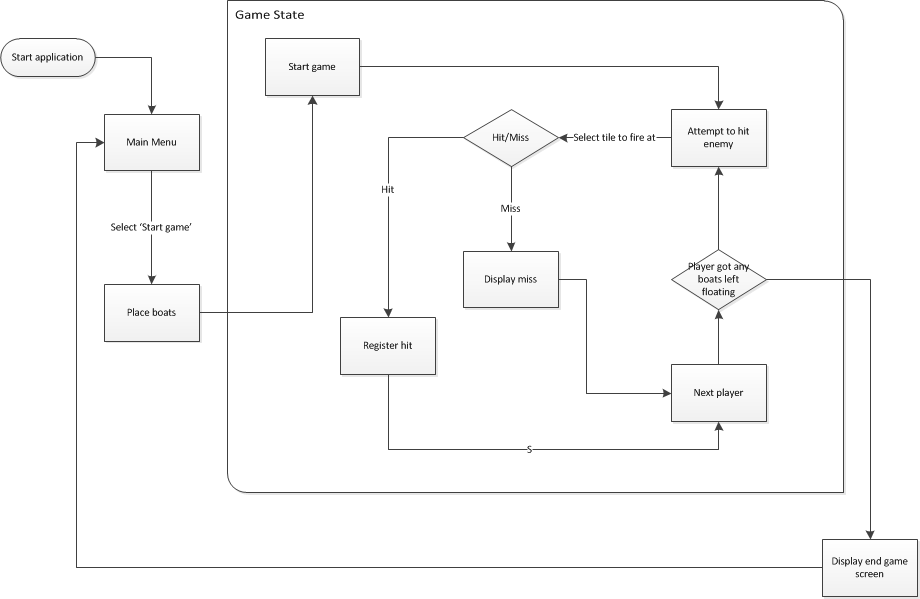
\includegraphics[angle=90, scale=0.8]{ProcessLayer.png}
    \caption{Process View Activity Diagram}
    \label{fig:ActivityDiagram}
\end{figure}

Figure \ref{fig:ActivityDiagram} shows an activity diagram describing the flow between the different actions and states.

When a player wants to start a game, the player will be be presented with the game's main menu. From here, the player will be able to choose \emph{Start game}, where, after placing its boats, the game will enter the main \emph{Game State}.

As soon as both of the players are ready, the game starts. Now the players will take turns in shooting at their opponents ships. This is done by having the first player select one of the opponent's tiles to bomb it. If the tile does not contain a warship, the game registers the miss and calculates data accordingly, and executes a turn switch activity, and the first player has to wait for the opponent to have a go at guessing his warships' placement.

If the tile did contain a warship, the game registers this as a hit and process data accordingly. If the last tile of the last warship was hit the game ends and declares the bombing player as the winner and exits.

Note that the diagram is a simplified version, and does not show the user customisation part\footnote{E.g. selection of player colour and setting a player name.} of the application. This would have been available from the \emph{Main Menu} activity.

